\section{Computer Software Design}
In this section we will cover a portion of the software design. Please refer to the source code available on GitHub for more details. 

\href{https://github.com/JaidenK/ME309\_Spring2025\_Project}{https://github.com/JaidenK/ME309\_Spring2025\_Project}

\subsection{Functional Requirements}
By this point we have a set of test data ready to be processed and a mathematical model that we would like to fit to that data. Before we write the code, we must define the requirements of the software. 

\begin{itemize}

\item Data Input

The software shall read in timestamped position data from a comma-separated-values text file. 

\item Test Description Database 

A method for the software to store descriptions and initial model parameters for each test shall be provided. 

\item Model Fitting

The software shall generate a trajectory model fitted to a subset of the sampled data. The fit shall minimize the square of the residuals.

\item Impact Location Prediction

The software shall estimate the impact location using the model. 

\item Plot Generation

The software will need to generate plots of various system properties, including but not limited to the position, velocity, and acceleration of the projectile. 

\end{itemize}

\subsection{Design Requirements}

The design of the code should strive to satisfy the following requirements.

\begin{itemize}

\item Modularity and Maintainability

Code will be module so that it can be be unit tested in isolation and to reduce coupling between code components. Code will be written with maintainability in mind so that we can re-use our code for future projects. In particular, the implementation of the model should be easily swappable. 

\item Generic Processing 

Code will not be tailored for specific test cases. Other than changing options, such as which data set to plot and which model type to use, there will be no need to modify code to get it to run properly between different data sets.

\end{itemize}

\subsection{System Design}
\begin{figure}[t]
\centering
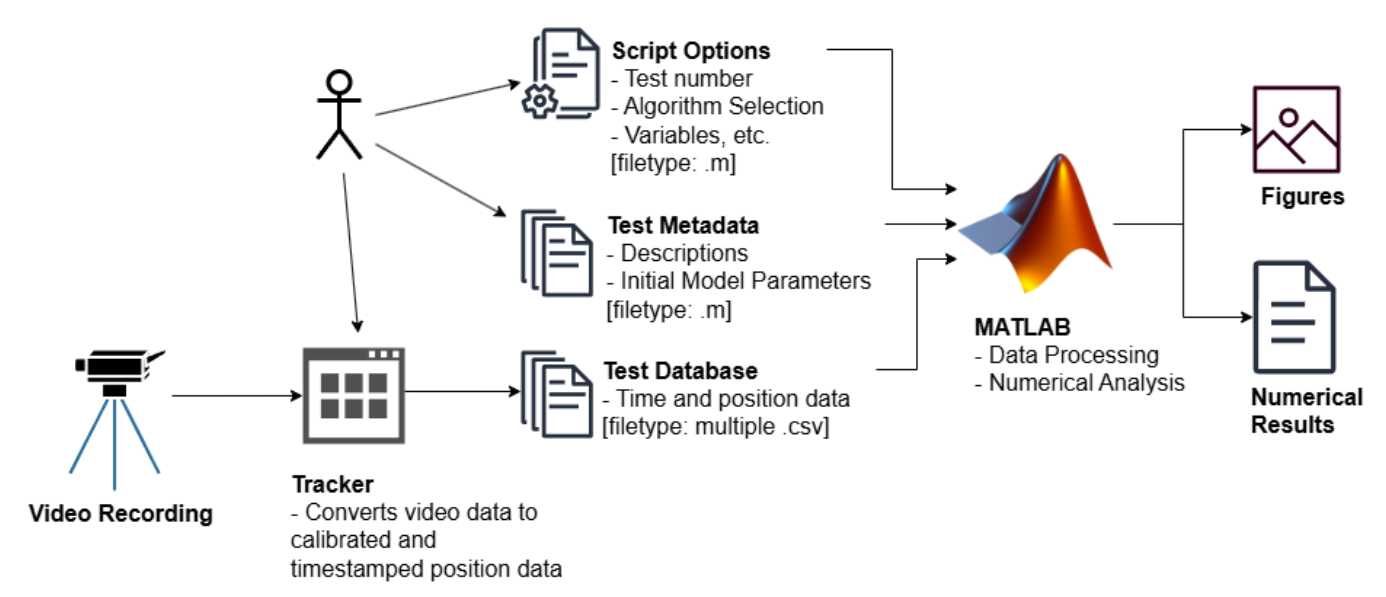
\includegraphics[width=0.9\linewidth]{images/SystemDiagram.png}
\caption{\label{fig:SystemDiagram} Software system diagram.}
\end{figure}

The system diagram shown in Fig.~\ref{fig:SystemDiagram} shows how the MATLAB scripts fit in to the system. We have several video clips, one per toss of the projectile, and each is processed by the user using Tracker. This provides us with multiple independent CSV files, which we called the Test Database. Next, we have the meta data describing each test, such as a plain text description and the initial model parameters. This is stored in a switch statement in the source code. Finally, all the configuration options are grouped into a single Script Options file. 

\begin{figure}[t]
\centering
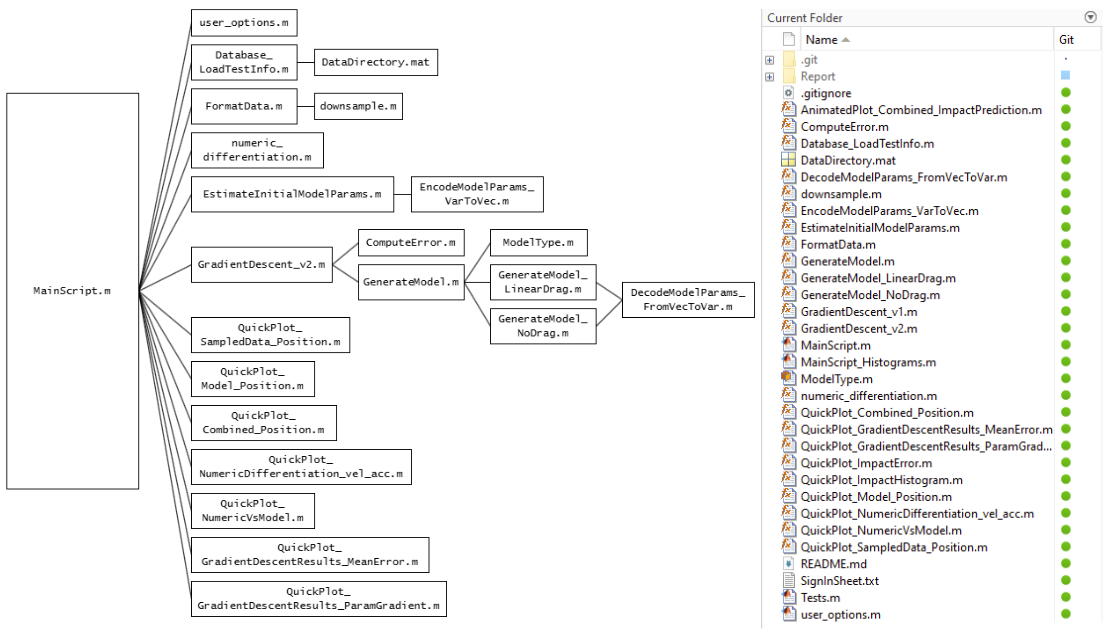
\includegraphics[width=0.9\linewidth]{images/MainScriptDiagram.png}
\caption{\label{fig:MainScriptDiagram} Main Script Diagram.}
\end{figure}

All of the inputs are used by the top level executable MATLAB script \texttt{MainScript.m}. Fig.~\ref{fig:MainScriptDiagram} attempts to show the relationships between the main script and the others. 

\section{Algorithms and Patterns}
Here we will highlight a few of the algorithms and coding patterns used. Again, the reader is encouraged to refer to the source code available on GitHub.

\subsection{Model Factory}
We knew that the Model implementation would change (going from a parabolic model to a linear drag model) while the interface to the model would remain unchanged (still has the same parameters and the output is just the equations of motion). We also wanted to be able to easily change which model we were using without editing all the lines of code referring to the model. To address this, we took inspiration from the Factory Pattern. The \texttt{GenerateModel.m} file implements the model factory, which returns the appropriate version of the model based on the provided function parameters.

\subsection{Numeric Differentiation}
Previously we had stated that the parabolic model would be used as a baseline. However, we can be even more based. Without using any specific model, we can use numeric differentiation to estimate the velocity and acceleration of the projectile from the position data. That is, calculating the velocity from the simple change in sampled position over change in time.

\begin{align*}
\text{velocity} = \frac{\Delta \text{position}}{\Delta \text{time}}
\end{align*}

And likewise for acceleration. 

This technique is included as a "reference signal" because it is frequently the default go-to technique for computing velocity and acceleration in real-time settings. Many engineers will likely encounter data computed in this way, so it should be familiar. As you'll see in the analysis sections, this technique is highly sensitive to noise in the signal. One of the advantages of using the model of best fit is that we can "see through" the noise.

\subsection{Gradient Descent}
The method used to fit our model to the sampled data is a custom variant of Gradient Descent. The Wikipedia article\footnote{\href{https://en.wikipedia.org/wiki/Gradient\_descent}{https://en.wikipedia.org/wiki/Gradient\_descent}} goes into greater detail and we will just summarize it here. In general, Gradient Descent allows you to find the minimum value of a function by sampling the gradient (i.e. slope) at some point and taking a small step "downhill". This is an iterative process where you just keep taking small steps downhill. The function we are minimizing is the sum of squared errors, where the error function is the difference between the sampled position and the model predicted position at that sample time. 

In our system this is a 5-dimensional landscape that we're walking downhill in. The 5 dimensions (the model parameters) are the initial position's x and y coordinates, initial velocity x and y coordinates, and the drag coefficient. 

Our special tweak to the algorithm was to, at each iteration, find the value of the drag coefficient which minimized the error. The gradient of the error function was then used to update the remaining 4 parameters. The implementation of this tweaked version is available in \texttt{GradientDescent\_v2.m}.

The reason we went with Gradient Descent is because it's known to converge even for non-linear systems, and we wanted a technique that would be applicable to as wide a variety of model types as possible. It's definitely possible we could improve the algorithms by linearizing the error function. 
